% !TEX program = xelatex

\documentclass{resume}
\usepackage{graphicx}
\usepackage{tabu}
\usepackage{multirow}
\usepackage{progressbar}
\usepackage{zh_CN-Adobefonts_external} % Simplified Chinese Support using external fonts (./fonts/zh_CN-Adobe/)
%\usepackage{zh_CN-Adobefonts_internal} % Simplified Chinese Support using system fonts
\begin{document}
\pagenumbering{gobble} % suppress displaying page number


\renewcommand{\arraystretch}{1.2}
\Large{
  \begin{tabu}{ c l l }
    \multirow{-2.4}{1in}{\vspace{-0.5in}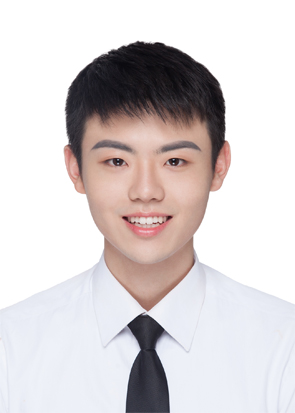
\includegraphics[width=0.95in]{pic}} & \scshape{陈欣祺} \hspace{1pt} 1998.08.28
    & \email{chenxq66@sjtu.edu.cn} \\
    & \phone{(+86) 150-130-20347} & \address{广东省深圳市}  \\
    & \homepage[https://master-chen-xin-qi.github.io/]{https://master-chen-xin-qi.github.io/} & \github[Master-Chen-Xin-Qi]{https://github.com/Master-Chen-Xin-Qi} \\
  \end{tabu}
}


% \Large{
%   \begin{tabu}{ c l r }
%    \multirow{5}{1in}{\includegraphics[width=0.88in]{avatar}} & \scshape{Bin Yuan} & {Python~}\progressbar{0.75} \\
%     & \email{yuanbin2014@gmail.com} & {Scala~}\progressbar{0.5} \\
%     & \phone{(+86) 131-221-87xxx} & {Linux~}\progressbar{0.7} \\
%     & \linkedin[billryan8]{https://www.linkedin.com/in/billryan8} & {Flask~}\progressbar{0.5} \\
%     & \github[github.com/billryan]{https://github.com/billryan} & {Javascript~}\progressbar{0.5}
%   \end{tabu}
% }

\large{}
\section{\faGraduationCap\ 教育经历}
\datedsubsection{\textbf{上海交通大学}, 上海}{2021.09 -- 2026.06}
\textit{博士},计算机科学与技术 \hspace{1.52cm} GPA: 3.8/4.0 (前10\%)
\datedsubsection{\textbf{中山大学}, 广州}{2017.09 -- 2021.06}
\textit{本科},电子信息科学与技术 \hspace{1.10cm} GPA: 3.9/5.0 (前10\%)

\section{\faUsers\ 实习经历}
\datedsubsection{\textbf{香港中文大学,计算机科学与工程系}}{2025.03 -- 2026.03}
\role{访问学生}{导师: Patrick P.C. Lee}
设计并开发一个块存储镜像数据预加载的算法,可以大幅减少系统盘冷启动的延迟。
% 提升serverless等应用的性能。

\datedsubsection{\textbf{阿里云,块存储团队} \hspace{4.18cm}}{2023.09 -- 2025.03}
\role{阿里巴巴研究型实习生}{主管: 徐尔茨}
为阿里云块存储设计并开发了一个proactive和reactive策略相结合的流量转发层调度器,Omar,与现有算法相比可以提升60\%的尾部延迟性能,并且可以减少50\%的调度次数。

\datedsubsection{\textbf{阿里云,盘古团队} \hspace{4.6cm}}{2022.07 -- 2023.09}
\role{阿里巴巴研究型实习生}{主管: 徐尔茨}
为阿里云盘古团队设计并开发了一个基于强化学习的归档存储调度器MasterPlan,与现有算法相比,可以提升1.25倍的吞吐,减少1.47倍的能耗,并减少2.16倍的尾部延迟。

% \datedsubsection{\textbf{普渡机器人,算法团队} \hspace{3.76cm} 深圳,广东}{2020.10 -- 2021.01}
% \role{算法实习生}{主管: 郭璁}
% 基于机器人的RGB-D相机设计并开发一个小目标检测算法。

\section{\faFileTextO \ 发表论文}
\begin{itemize}[parsep=0.5ex]
  \item \textbf{Xinqi Chen}, Weidong Zhang, Zhongyu Wang, Erci Xu, Dong Wu, Xiaolu Zhang, Haonan Wu, Yaheng Song, Chaolei Hu, et al. Come for the QoS? Load Best Not Be Balanced! Scheduling Cloud Block Store Proactively and Reactively with
  Omar. (\textbf{CCF A, In submission}). 2025.
  \item Lanqing Yang, \textbf{Xinqi Chen}, Hao Pan, Yi-Chao Chen, Guangtao Xue, Zechen Li, et al. MagPrint++: Continuous User Fingerprinting On
  Mobile Devices Using Electromagnetic Signals. \textit{IEEE Transaction on Mobile Computing} (\textbf{CCF A, Major Revision}). 2025.
  \item \textbf{Xinqi Chen}, Erci Xu, Dengyao Mo, Ruiming Lu, Haonan Wu, Dian Ding, Guangtao Xue. MasterPlan: A Reinforcement Learning Based Scheduler for Archive Storage. \textit{ACM Transaction on Architecture and Code Optimization} (\textbf{CCF A}). 2024.
  \item Haonan Wu, Erci Xu, Ligang Wang, Yuandong Hong, Changsheng Niu, Bo Shi, Lingjun Zhu, Jinnian He, Dong Wu, Weidong Zhang, Qiuping Wang, Changhong Wang, \textbf{Xinqi Chen}, Guangtao Xue, Yi-Chao Chen, Dian Ding. Hey Hey, My My, Skewness Is Here to Stay: Challenges and Opportunities in Cloud Block Store Traffic. \textit{ACM EuroSys} (\textbf{CCF A}). 2024.
  \item Lanqing Yang, \textbf{Xinqi Chen}, Xiangyong Jian, Leping Yang, Yijie Li, Qianfei Ren, Yi-Chao Chen, Guangtao Xue, Xiaoyu Ji. Remote Attacks on Speech Recognition Systems Using Sound from Power Supply. \textit{USENIX Security Symposium} (\textbf{CCF A}). 2023.
\end{itemize}


% Reference Test
%\datedsubsection{\textbf{Paper Title\cite{zaharia2012resilient}}}{May. 2015}
%An xxx optimized for xxx\cite{verma2015large}
%\begin{itemize}
%  \item main contribution
%\end{itemize}

% \section{\faCogs\ Skills}
% \begin{itemize}[parsep=0.5ex]
%   \item Programming Languages: C == Python > C++ > Java
%   \item Platform: Linux
%   \item Development: Web, xxx
% \end{itemize}

% \section{\faHeartO\ Honors and Awards}
% \datedline{\textit{\nth{1} Prize}, Award on xxx }{Jun. 2013}
% \datedline{Other awards}{2015}

\section{\faCogs\ 其他}
\begin{itemize}[parsep=0.5ex]
  \item 技能:Python, C/C++, Golang, Latex, SQL, Shell, Linux, Docker
  \item 语言:中文(母语),英文(CET-6 564)
  \item 科研服务:ICIC 2024(审稿人)
\end{itemize}

%% Reference
%\newpage
%\bibliographystyle{IEEETran}
%\bibliography{mycite}
\end{document}
